\newpage
\section*{Nord}
\label{nord}

\phantomsection
\addcontentsline{toc}{section}{Nord}
\thispagestyle{empty}

\begin{center} 
\textbf{Open Composition Opus 2}
\label{oco2}

{\scriptsize  \texttt{Copyleft \textcopyleft \, 2017 Yann Ics - All Wrongs Reserved.}}
 \end{center} 
\vspace{-5mm}
\subsection*{\quad Chord diagrams}
\vspace{-5mm}
 \begin{figure}[H]
\begin{center}
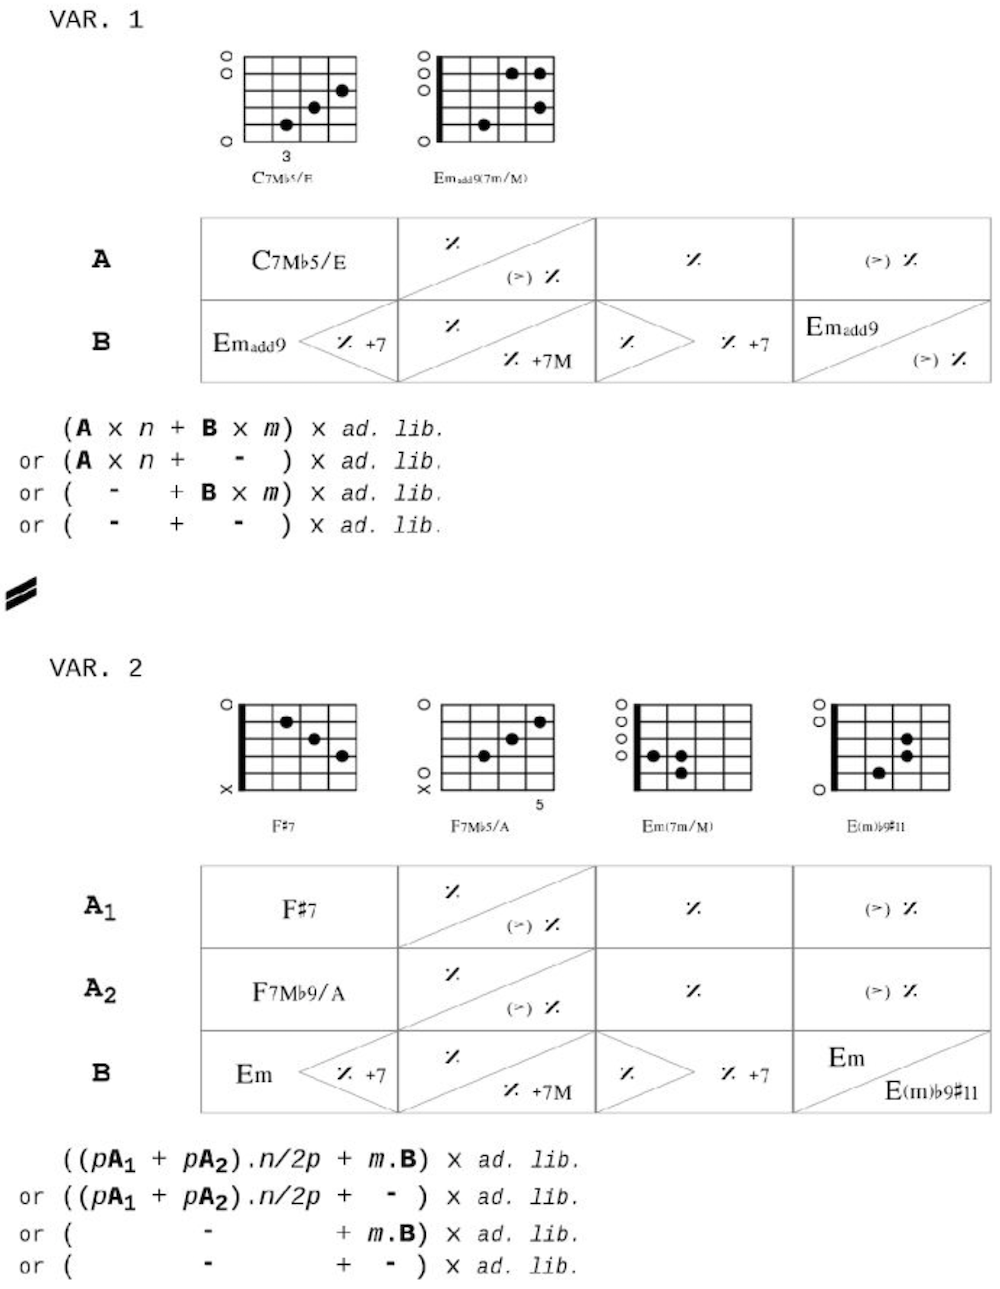
\includegraphics[scale=0.66]{img/tn1}
\end{center}
\end{figure}


 \begin{figure}[H]
\begin{center}
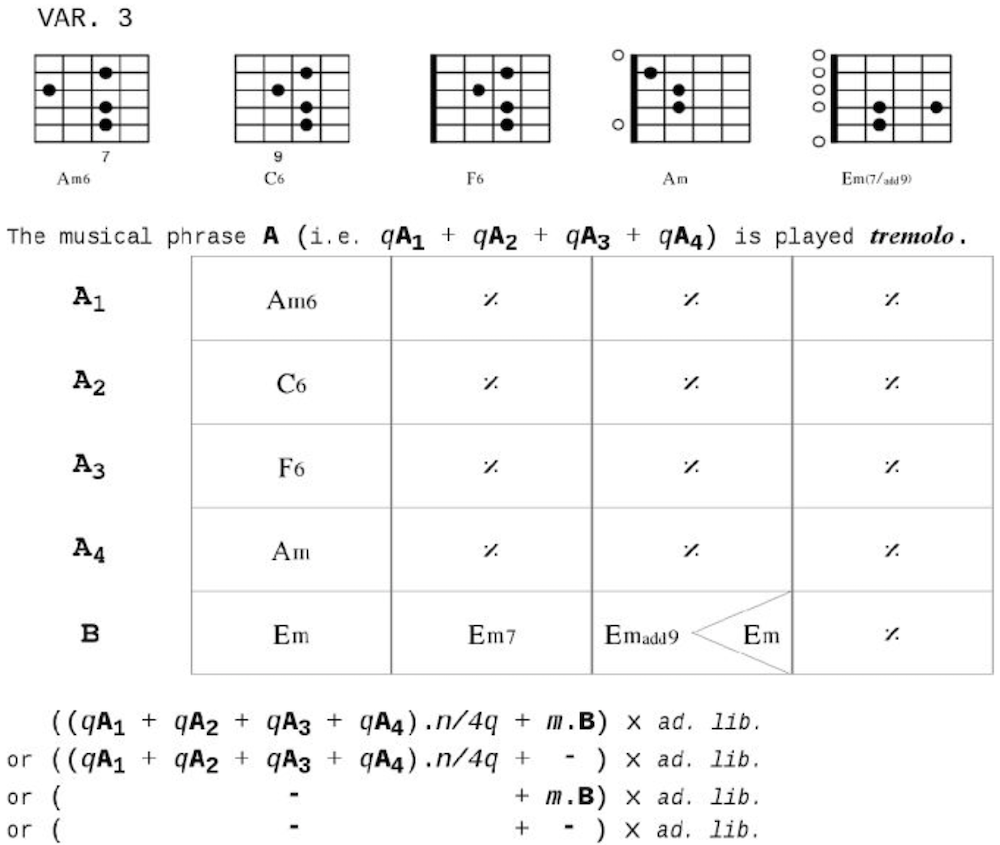
\includegraphics[scale=0.66]{img/tn2}
\end{center}
\end{figure}

\bigskip

\subsection*{\quad Interlude}
\label{interlude}

\bigskip

Interlude is the part of Nord written in tablature for two guitars. In fact, there are two distinct parts, therefore two interludes, but which are thematically interconnected. So there is an interlude called \textsl{Nomad} composed of three movements, the last movement of which is played as a soloist; and a more autonomous interlude called \textsl{Monkey}, which can be played repeatedly, and even mixed in at any moment during the performance. 

\bigskip 

The cells marked A and B (see also A' and B' for the \textsl{Monkey} interlude) in the scores can be played \textit{ad libitum}, being able to serve as digressions or to support a possible interaction depending on the context. Along the same lines, the use of a wind instrument is particularly encouraged.

\bigskip

The dynamic aspect must be considered according to the interpreter's feelings. Last, all notes and open strings must resonate as long as possible, more or less understood like a \textit{legatissimo}.
\newpage

 \quad \textbf{\textsl{Nomad}} Movement 1 

\smallskip

 \quad \quad Guitar 1

\begin{center}
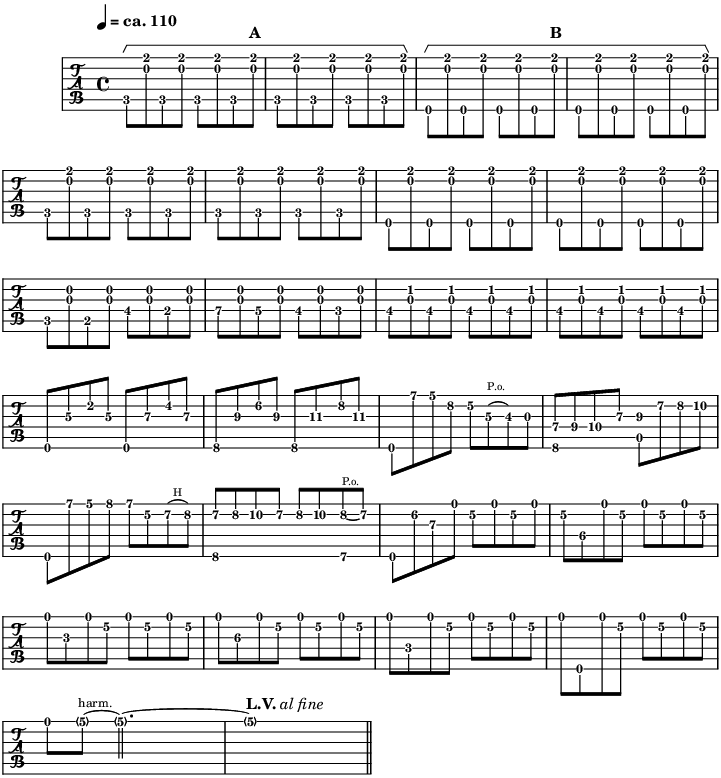
\includegraphics[scale=0.5]{img/neA1}
\end{center}

 \quad \quad Guitar 2

\begin{center}
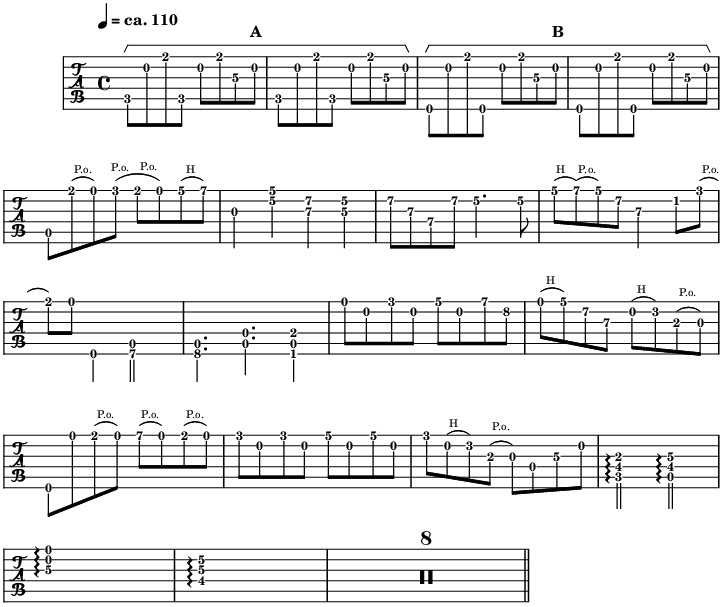
\includegraphics[scale=0.5]{img/neA2}
\end{center}

\newpage

\quad \quad \textbf{\textsl{Nomad}} Movement 2 

\smallskip

\quad \quad \quad Guitar 1

\begin{center}
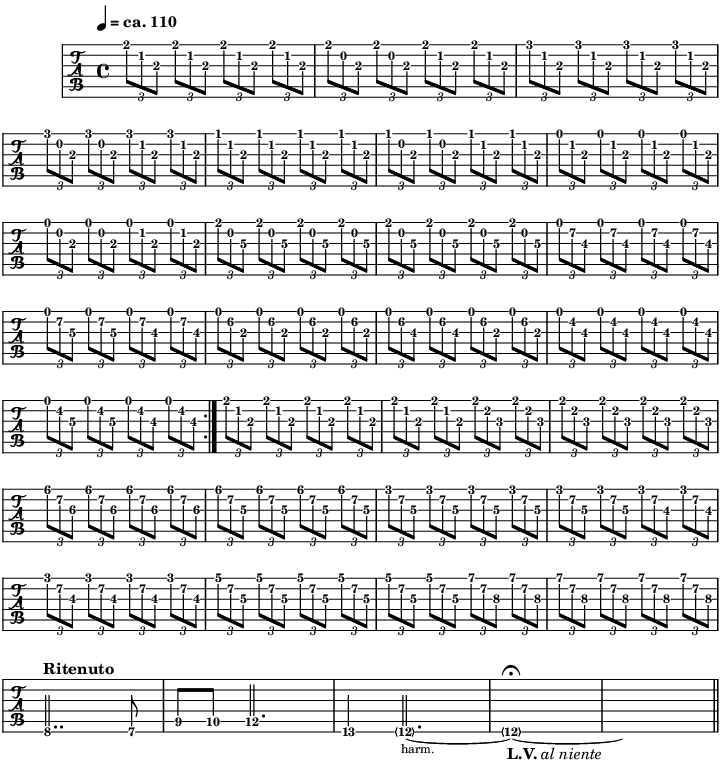
\includegraphics[scale=0.45]{img/neB1}
\end{center}

\quad \quad \quad Guitar 2

\begin{center}
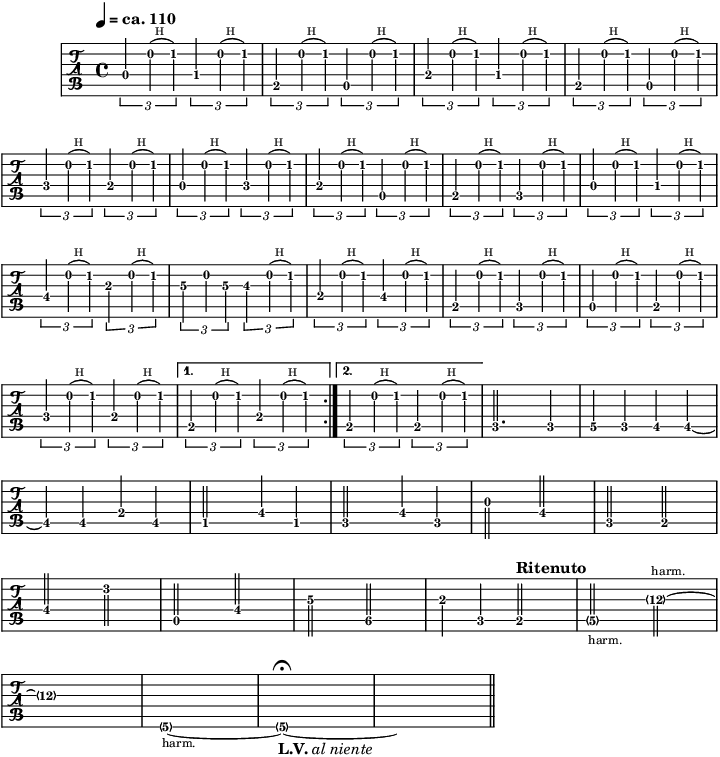
\includegraphics[scale=0.45]{img/neB2}
\end{center}

\newpage

 \textbf{\textsl{Nomad}} Movement 3 

\smallskip

 \quad Guitar solo

\begin{center}
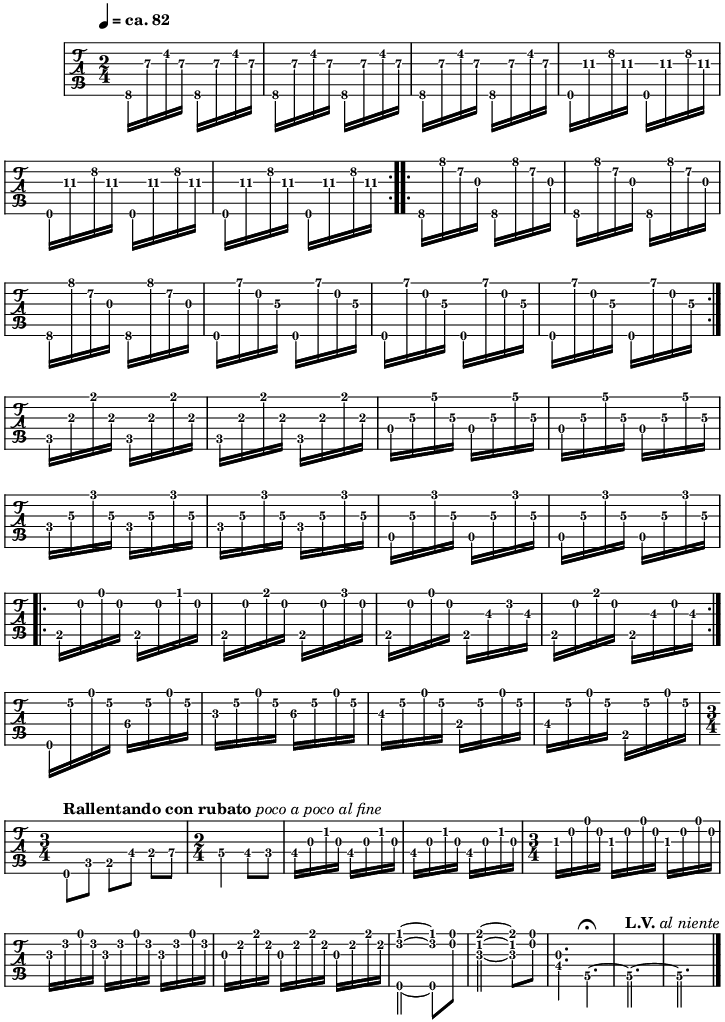
\includegraphics[width=\textwidth]{img/neC1}
\end{center}

\newpage

\textbf{\textsl{Monkey}}  

\smallskip

 \quad Guitar 1

\begin{center}
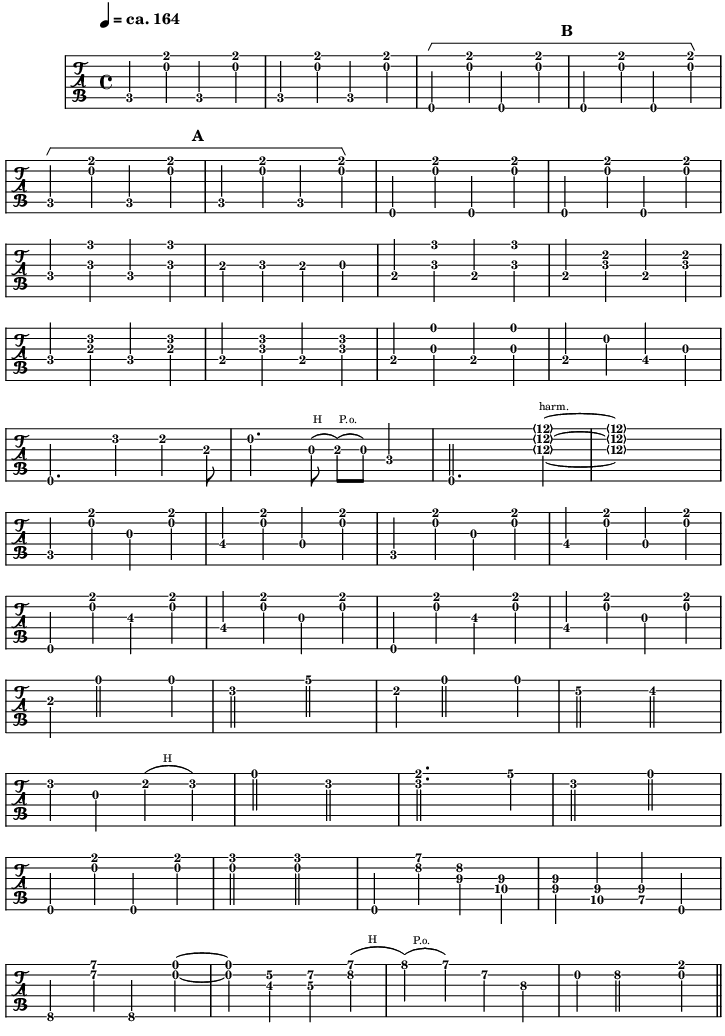
\includegraphics[width=\textwidth]{img/neD1}
\end{center}

\newpage
\textbf{\textsl{Monkey}}  

\smallskip

 \quad Guitar 2
 
\begin{center}
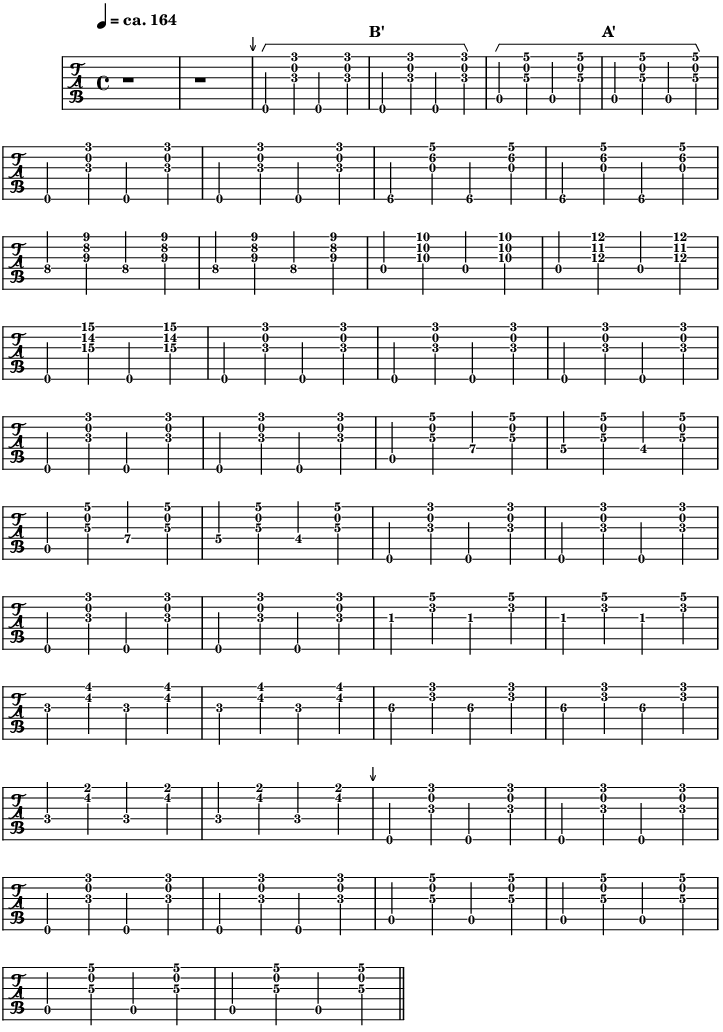
\includegraphics[width=\textwidth]{img/neD2}
\end{center}
